\documentclass[12pt, a4paper]{article}

% ==========================================
% 1. KHAI BÁO GÓI THƯ VIỆN (PACKAGES)
% ==========================================
% Bảng mã & Font chữ
\usepackage[utf8]{inputenc}
\usepackage[T5]{fontenc}

% Toán học
\usepackage{amsmath, amssymb}

% Căn lề & Bố cục trang
\usepackage[top=2.2cm, bottom=1.5cm, left=1cm, right=1cm, headheight=15pt]{geometry}
\usepackage{fancyhdr}
\usepackage{needspace}
\usepackage{tkz-tab}
\usepackage{float}

% Đồ họa & Màu sắc
\usepackage{xcolor}
\usepackage{graphicx} 
\usepackage{tikz}
\usetikzlibrary{calc, shapes.geometric, positioning}


% Bảng biểu & Danh sách
\usepackage{colortbl}
\usepackage{array}
\usepackage{makecell}
\usepackage{multirow}
\usepackage{tasks}

% Biểu tượng
\usepackage{fontawesome5}

% ==========================================
% 2. THIẾT LẬP MÀU SẮC CHỦ ĐẠO
% ==========================================
\definecolor{goldyellow}{RGB}{255, 179, 0}
\definecolor{amberorange}{RGB}{230, 115, 0}
\definecolor{lightamber}{RGB}{255, 248, 225}
\definecolor{deepblue}{RGB}{25, 42, 86}
\definecolor{accentred}{RGB}{232, 65, 24}
\definecolor{softgray}{RGB}{220, 220, 222} 
\definecolor{fbblue}{RGB}{15, 80, 200}


% ==========================================
% 3. CẤU HÌNH HEADER & FOOTER
% ==========================================
\pagestyle{fancy}
\fancyhf{}
\renewcommand{\headrulewidth}{0pt}

% Khai báo biến lưu trữ nội dung góc phải của Header
\newcommand{\HeaderRightText}{}

% --- Header ---
\fancyhead[C]{
    \begin{tikzpicture}[remember picture, overlay]
        
        % Dải màu trang trí góc trên
        \path[fill=deepblue] (current page.north west) -- (current page.north east) 
            -- ($(current page.north east) + (0, -1.6cm)$) 
            .. controls ($(current page.north) + (3, -2.0cm)$) and ($(current page.north) + (-3, -0.4cm)$) .. 
            ($(current page.north west) + (0, -1.0cm)$) -- cycle;
            
        \path[fill=goldyellow] (current page.north west) -- (current page.north east) 
            -- ($(current page.north east) + (0, -1.0cm)$) 
            .. controls ($(current page.north) + (4, -1.0cm)$) and ($(current page.north) + (-2, -2.2cm)$) .. 
            ($(current page.north west) + (0, -1.6cm)$) -- cycle;
            
        \path[fill=amberorange] (current page.north west) -- ($(current page.north west) + (6.5cm, 0)$) 
            .. controls ($(current page.north west) + (4.5cm, -1.2cm)$) and ($(current page.north west) + (2cm, -2.0cm)$) .. 
            ($(current page.north west) + (0, -2.0cm)$) -- cycle;
            
        % Logo góc trái Header
        \node[anchor=west, inner sep=0pt] 
            at ($(current page.north west) + (0cm, -0.8cm)$) {
\includegraphics[height=2.0cm]{../../../image/logo-header.png}};
            
        % Text góc phải Header (Tự động lấy từ đối số thứ 3 của \titlebox)
        \node[anchor=east, text=white, font=\small\bfseries\sffamily] 
            at ($(current page.north east) + (-0.8cm, -0.5cm)$) {\HeaderRightText};
    \end{tikzpicture}
}

% --- Footer ---
\fancyfoot[C]{
    \begin{tikzpicture}[remember picture, overlay]
        % Đường kẻ ngang
        \draw[amberorange, line width=1.5pt] 
            ($(current page.south west) + (0cm, 0.4cm)$) -- ($(current page.south east) + (0cm, 0.4cm)$);

        % Dải cong góc phải
        \path[fill=goldyellow] (current page.south east) -- ($(current page.south east) + (-5cm, 0)$) 
            .. controls ($(current page.south east) + (-3cm, 0.8cm)$) and ($(current page.south east) + (-1.5cm, 1.2cm)$) .. 
            ($(current page.south east) + (0, 1.2cm)$) -- cycle;

        % Mạng xã hội
        \node[anchor=west, inner sep=0pt] at ($(current page.south west) + (1cm, 0.8cm)$) {
            \small\sffamily
            \textcolor{fbblue}{\faFacebook\hskip 4pt Toán Anh Huy MATH-STER}
            \hskip 18pt
            \textcolor{black}{\faTiktok\hskip 4pt huymathster}
        };

        % Số trang
        \node[circle, fill=white, draw=amberorange, line width=1.5pt, text=deepblue, font=\large\bfseries\sffamily, inner sep=4pt, minimum size=0.8cm] 
            at ($(current page.south east) + (-1.2cm, 0.6cm)$) {\thepage};
    \end{tikzpicture}
}

% ==========================================
% 4. ĐỊNH NGHĨA MACRO: KHUNG TIÊU ĐỀ
% ==========================================
\newcommand{\titlebox}[3]{
    % Gán nội dung đối số #3 vào biến HeaderRightText
    \gdef\HeaderRightText{#3}
    
    \begin{center}
    \vspace*{-0.5cm}
    \begin{tikzpicture}
        % Khung vô hình (Phantom Box) định chuẩn kích thước
        \node[text width=16cm, inner xsep=0pt, inner ysep=16pt, opacity=0] (MainBox) {
            \begin{minipage}[c]{4.2cm}
                \centering\vspace{0.1cm}
                \rule{2.2cm}{2.2cm} 
                \vspace{0.1cm}
            \end{minipage}%
            \begin{minipage}[c]{11.5cm}
                \centering\vspace{0.15cm}
                {\huge\bfseries\sffamily #2 \par}
                \vspace{0.15cm} 
            \end{minipage}
        };
        
        % Đổ bóng & Nền
        \fill[goldyellow, rounded corners=8pt] ([xshift=5pt, yshift=-5pt]MainBox.south west) rectangle ([xshift=5pt, yshift=-5pt]MainBox.north east);
        \fill[white, rounded corners=8pt] (MainBox.south west) rectangle (MainBox.north east);
        
        % Lưới ô ly & Nền Logo
        \begin{scope}
            \clip[rounded corners=8pt] (MainBox.south west) rectangle (MainBox.north east);
            \draw[step=0.4cm, softgray!50, line width=0.6pt] (MainBox.south west) grid (MainBox.north east);
            \fill[lightamber!60] (MainBox.south west) rectangle ([xshift=4.2cm]MainBox.north west);
        \end{scope}

        % Viền ngoài
        \draw[deepblue, line width=1.5pt, rounded corners=8pt] (MainBox.south west) rectangle (MainBox.north east);

        % Nội dung Text (Lớp trên cùng)
        \node[text width=16cm, inner xsep=0pt, inner ysep=16pt] at (MainBox.center) {
            \begin{minipage}[c]{4.2cm}
                \centering
                % --- ĐIỀU CHỈNH TỌA ĐỘ LOGO Ở ĐÂY ---
                \hspace*{-0.5cm}\raisebox{-0.2cm}{
\includegraphics[width=5.5cm]{../../../image/logo.png}}
            \end{minipage}%
            \begin{minipage}[c]{11.5cm}
                \centering\vspace{0.15cm}
                {\huge\bfseries\sffamily\color{deepblue} #2 \par}
                \vspace{0.15cm} 
            \end{minipage}
        };
        
        % Trang trí phụ kiện
        \draw[deepblue, line width=1.5pt, dashed] ([xshift=4.2cm]MainBox.north west) -- ([xshift=4.2cm]MainBox.south west);
        \node[regular polygon, regular polygon sides=4, rotate=45, fill=white, draw=accentred, line width=1.2pt, inner sep=2.5pt] at ([xshift=4.2cm]MainBox.west) {};
        \node[anchor=west, fill=amberorange, text=white, font=\large\bfseries\sffamily, rounded corners=4pt, draw=deepblue, line width=1.5pt, inner xsep=12pt, inner ysep=6pt] at ([xshift=1.5cm]MainBox.north west) {#1};
        \fill[accentred] ([xshift=-1.8cm, yshift=-0.4cm]MainBox.north east) circle (3pt);
        \fill[amberorange] ([xshift=-1.4cm, yshift=-0.4cm]MainBox.north east) circle (3pt);
        \fill[goldyellow] ([xshift=-1.0cm, yshift=-0.4cm]MainBox.north east) circle (3pt);
    \end{tikzpicture}
    \vspace*{0cm}
    \end{center}
}

% ==========================================
% 5. ĐỊNH NGHĨA MACRO: CẤU TRÚC CÂU HỎI (ÉP SÁT NHAU)
% ==========================================
\newcommand{\questioncore}[2]{
    % Xóa khoảng cách phía trên, ép sát câu trước
    \noindent \textbf{\textcolor{deepblue}{Câu #1.} \textcolor{accentred}{[STER]}} #2
    \par\nopagebreak
}

% Cấu hình hiển thị đáp án trắc nghiệm
\settasks{
    label=\textbf{\textcolor{amberorange}{\Alph*.}}, 
    label-width=15pt,     
    item-indent=25pt,     
    label-offset=6pt,    
    column-sep=20pt,     
    after-item-skip=2pt  % Đã giảm tối đa khoảng cách giữa các dòng đáp án A B C D
}

% Hàm vẽ dòng kẻ nháp
\newcommand{\drawdashlines}[1]{
    \ifnum#1>0
        \nopagebreak\vspace{0.1cm}\noindent 
        \begin{tikzpicture}
            \foreach \i in {1,...,#1} {
                \draw[softgray, line width=0.2pt] (0,-{\i*0.75}) -- (\textwidth-4pt,-{\i*0.75});
            }
        \end{tikzpicture}
        \par
    \fi
    % Đã xóa hoàn toàn khoảng cách thừa ở nhánh else
}

% --- Dạng 1: Trắc nghiệm 4 đáp án ---
\newcommand{\questionLinesManual}[4]{
    \pgfmathsetmacro{\calculatedSpace}{1.5 + #1 * 0.65}
    \needspace{\calculatedSpace cm} 
    \questioncore{#2}{#3}
    #4
    \par\nopagebreak
    \drawdashlines{#1}
}
% --- Dạng 2: Trắc nghiệm Đúng/Sai ---
\newcommand{\questionTrueFalse}[4]{
    \scriptsize
    \pgfmathsetmacro{\calculatedSpace}{3.0 + #1 * 0.65} 
    \needspace{\calculatedSpace cm}
    \questioncore{{#2}}{#3}
    
    \nopagebreak
    \begin{flushleft}
    \renewcommand{\arraystretch}{1.2} % Bóp nhỏ chiều cao của bảng Đ/S
    \begin{tabular}{|>{\centering\arraybackslash}m{0.4cm}|m{6cm}|>{\centering\arraybackslash}m{1cm}|>{\centering\arraybackslash}m{1cm}|}
        \hline
        \rowcolor{amberorange!20}
        & \multicolumn{1}{>{\centering\arraybackslash}m{6cm}|}{\textbf{\textcolor{deepblue}{Mệnh đề}}} & 
        \textbf{\textcolor{deepblue}{Đúng}} & 
        \textbf{\textcolor{deepblue}{Sai}} \\
        \hline
        #4
        \hline
    \end{tabular}
    \renewcommand{\arraystretch}{1}
    \end{flushleft}
    
    \par\nopagebreak
    \drawdashlines{#1}
}

% ----- Dạng 3: Tự luận ngắn -----
\newcommand{\questionShortAnswer}[3]{
    \scriptsize
    \pgfmathsetmacro{\calculatedSpace}{1.5 + #1 * 0.8}
    \needspace{\calculatedSpace cm}
    
    {\linespread{1.1}\selectfont % Bóp nhỏ giãn dòng của câu tự luận
    \questioncore{#2}{#3}\par}
    
    \nopagebreak
    \begin{flushright}
        \begin{tikzpicture}
            \node[anchor=east, font=\small\bfseries\sffamily, text=deepblue] 
                at (-0.2, 0.4) {Đáp án:};
            \fill[goldyellow, rounded corners=3pt] (0.08, -0.08) rectangle (3.08, 0.72);
            \draw[draw=deepblue, fill=white, line width=1.2pt, rounded corners=3pt] 
                (0,0) rectangle (3.0, 0.8);
            \foreach \x in {0.75, 1.5, 2.25} {
                \draw[draw=deepblue, line width=0.6pt] (\x, 0) -- (\x, 0.8);
            }
        \end{tikzpicture}
    \end{flushright}
    
    \par\nopagebreak
    \drawdashlines{#1}
}

% ==========================================
% BẮT ĐẦU NỘI DUNG TÀI LIỆU
% ==========================================
\begin{document}

% Truyền 3 tham số: {Nhãn cam} {Chữ to chính giữa} {Chữ ở góc phải Header}
\titlebox{Chủ đề: Hàm số}{BTDD min Max diện tích thể tích}{Hàm số: Min Max DT-TT}

\questionTrueFalse{20}{1}{Ông An cần xây dựng một bể chứa nước có dạng hình hộp chữ nhật không có nắp đậy để phục vụ cho việc tưới cây trong vườn. Do các điều kiện về diện tích vườn, ông An cần bể có thể tích là \( 24m^3 \), đáy bể có chiều dài gấp hai lần chiều rộng và chiều rộng không quá \( 4m \), biết rằng chi phí vật liệu xây dựng mỗi mét vuông diện tích bề mặt là \( 600\,000 \) đồng. Gọi \( x \, (m) \) là chiều rộng của bể, ta có \( 0 < x \leq 4 \). Khi đó:}{
    \textbf{a)} & Chiều cao của bể là \( \dfrac{12}{x^2} \, (m) \).
    & \textcolor{amberorange}{$\bigcirc$} & \textcolor{amberorange}{$\bigcirc$} \\ \hline
    
    \textbf{b)} & Tổng diện tích các mặt cần xây là \( 2x^2 + \dfrac{36}{x} \).
    & \textcolor{amberorange}{$\bigcirc$} & \textcolor{amberorange}{$\bigcirc$} \\ \hline
    
    \textbf{c)} & Để tổng chi phí vật liệu xây dựng là thấp nhất thì chiều cao của bể nước là \( h = \dfrac{2\sqrt[3]{18}}{3} \).
    & \textcolor{amberorange}{$\bigcirc$} & \textcolor{amberorange}{$\bigcirc$} \\ \hline
    
    \textbf{d)} & Ông An dự tính với ngân sách \( 24,5 \) triệu đồng thì sẽ đủ để ông có thể xây dựng bể chứa nước như mong muốn.
    & \textcolor{amberorange}{$\bigcirc$} & \textcolor{amberorange}{$\bigcirc$} \\
}

% --- CÂU 9 ---
\questionTrueFalse{20}{2}{Một tấm nhôm hình vuông cạnh 240 cm. Người ta cắt ở bốn góc của tấm nhôm đó bốn hình vuông bằng nhau, mỗi hình vuông có cạnh bằng \( x \) (cm), rồi gấp tấm nhôm lại như hình vẽ dưới đây để được một cái hộp không nắp.
\begin{center}
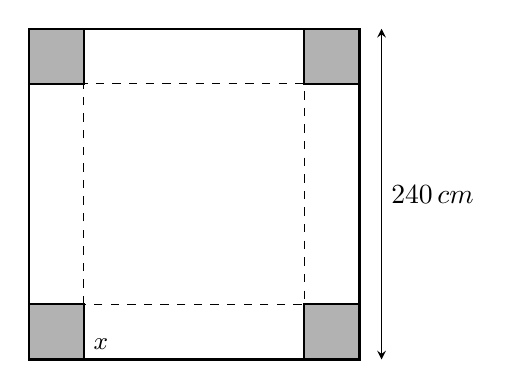
\begin{tikzpicture}[scale=0.35, >=stealth]
    % --- HÌNH 1: MẢNH CÁC TẤM BÌA PHẲNG ---
    % Khai báo kích thước tổng thể và cạnh cắt x
    \def\a{12}
    \def\x{2}
    
    % Tô màu xám cho 4 góc bị cắt
    \fill[gray!60] (0,0) rectangle (\x,\x);
    \fill[gray!60] (0,\a-\x) rectangle (\x,\a);
    \fill[gray!60] (\a-\x,0) rectangle (\a,\x);
    \fill[gray!60] (\a-\x,\a-\x) rectangle (\a,\a);
    \draw[thick] (0,0) rectangle (\x,\x);
    \draw[thick] (0,\a-\x) rectangle (\x,\a);
    \draw[thick] (\a-\x,0) rectangle (\a,\x);
    \draw[thick] (\a-\x,\a-\x) rectangle (\a,\a);
    % Vẽ biên ngoài hình vuông lớn
    \draw[thick] (0,0) rectangle (\a,\a);
    \draw[dashed] (\x,\x) rectangle (\a-\x,\a-\x);
   
    % Kí hiệu đoạn x ở góc
    \node at (\x, 0) [above right] {\small $x$};
    
    % Kí hiệu kích thước cạnh 12cm
    \draw[<->] (\a + 0.8, 0) -- (\a + 0.8, \a) node[midway, right] {$240\,cm$};
\end{tikzpicture}
\quad \quad \quad
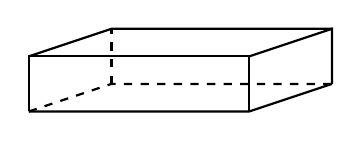
\begin{tikzpicture}[scale=0.35, >=stealth]
    % --- HÌNH 2: HÌNH HỘP CHỮ NHẬT 3D KHÔNG NẮP ---
    % Định nghĩa các điểm tọa độ mặt đáy
    \coordinate (A) at (0,0);
    \coordinate (B) at (8,0);
    \coordinate (C) at (11,1);
    \coordinate (D) at (3,1);
    
    % Chiều cao hộp h
    \def\h{2}
    
    % Các điểm mặt trên
    \coordinate (A1) at (0,\h);
    \coordinate (B1) at (8,\h);
    \coordinate (C1) at (11,3);
    \coordinate (D1) at (3,3);
    
    % Vẽ các nét khuất (nét đứt phía sau)
    \draw[dashed, thick] (A) -- (D) -- (C);
    \draw[dashed, thick] (D) -- (D1);
    
    % Vẽ các nét thấy phía trước và mặt trên mở
    \draw[thick] (A) -- (B) -- (C);
    \draw[thick] (A) -- (A1) -- (B1) -- (B);
    \draw[thick] (B1) -- (C1) -- (C);
    \draw[thick] (A1) -- (D1) -- (C1);
    
\end{tikzpicture}
\end{center}
}
{
    \textbf{a)} & Thể tích khối hộp nhận được khi tính theo \( x \) là  
    \(V = x(240 - 2x)^2.\)
    & \textcolor{amberorange}{$\bigcirc$} & \textcolor{amberorange}{$\bigcirc$} \\ \hline
    
    \textbf{b)} & Khi \( x = 20 \, cm \) thì thể tích của khối hộp nhận được là \( 8 \, m^3 \).
    & \textcolor{amberorange}{$\bigcirc$} & \textcolor{amberorange}{$\bigcirc$} \\ \hline
    
    \textbf{c)} & Để hộp nhận được có thể tích lớn nhất thì \( x = 60 \, cm \).
    & \textcolor{amberorange}{$\bigcirc$} & \textcolor{amberorange}{$\bigcirc$} \\ \hline
    
    \textbf{d)} & Hộp nhận được có thể tích lớn nhất là \( 1024 \, dm^3 \).
    & \textcolor{amberorange}{$\bigcirc$} & \textcolor{amberorange}{$\bigcirc$} \\
}

% --- CÂU 24 ---
\questionShortAnswer{20}{3}{Một người nông dân có 18 000 000 đồng để làm một hàng rào hình chữ \( E \) dọc theo một con sông bao quanh hai khu đất trồng rau có dạng hai hình chữ nhật bằng nhau (hình vẽ). Đối với mặt hàng rào song song với bờ sông thì chi phí nguyên vật liệu là 60 000 đồng/mét, còn đối với ba mặt hàng rào song song nhau thì chi phí nguyên vật liệu là 20 000 đồng/mét, mặt giáp với bờ sông không phải rào. Tìm diện tích lớn nhất của hai khu đất thu được sau khi làm hàng rào (đơn vị: ha).

\begin{center}
\begin{tikzpicture}[>=latex, scale=0.8]
    \begin{scope}[xshift=0cm, yshift=0cm]
        \node[anchor=south west, inner sep=0] at (0,0) {
            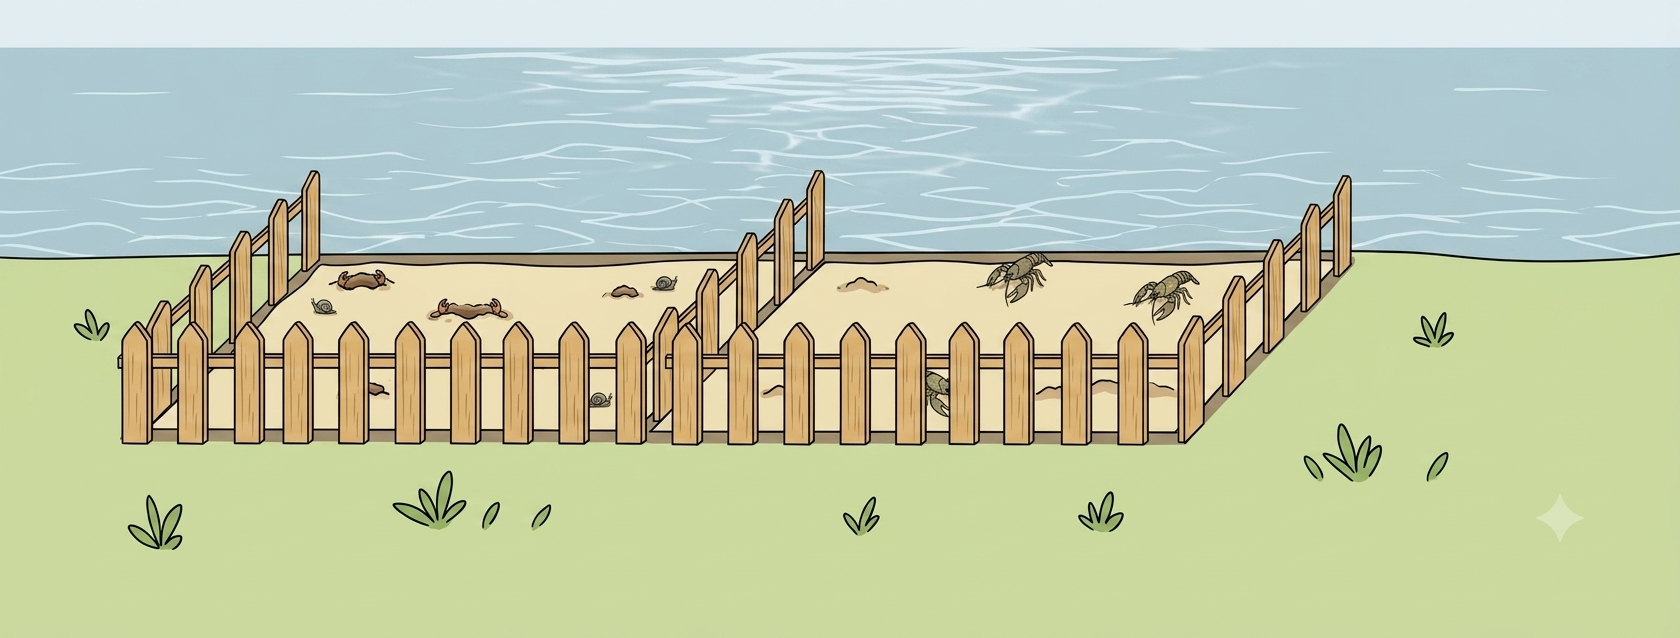
\includegraphics[width=5cm]{../images/HangRao.png}
        };
    \end{scope}
\end{tikzpicture}
\end{center}}


% --- CÂU 13 ---
\questionShortAnswer{20}{4}{Anh Tú dự định làm một cái thùng đựng nước hình trụ bằng nhôm có nắp đậy có thể tích \( 30 \, m^3 \). Chi phí làm mỗi \( m^2 \) đáy là 200 000 đồng, mỗi \( m^2 \) nắp là 100 000 đồng và mỗi \( m^2 \) mặt xung quanh là 150 000 đồng. Để chi phí làm thùng là thấp nhất thì anh Tú nên làm chiếc thùng với chiều cao là bao nhiêu mét? (Xem độ dài của tấm nhôm là không đáng kể, kết quả làm tròn đến hàng phần trăm).}


\end{document}